\documentclass[a4paper]{scrreprt}
    
%% Language and font encodings and page settings
\usepackage[english]{babel}
\usepackage[utf8x]{inputenc}
\usepackage[T1]{fontenc}
\usepackage[a4paper,top=2cm,bottom=2cm,left=3cm,right=3cm,marginparwidth=2cm]{geometry}
\usepackage{float}

%% Packages
\usepackage{amsmath}
\usepackage{graphicx}
\usepackage[colorinlistoftodos]{todonotes}
\usepackage[allcolors=blue]{hyperref}
\usepackage{wrapfig}
\graphicspath{{./img/}}

%% BibLaTeX settings
\usepackage[backend=biber]{biblatex}
\addbibresource{main.bib}

%% Header page information
\title{\href{https://github.com/cian2009/GestureReview}{Gesture Based User Interface Experience – Evolution and Challenges}}
\subtitle{"Gesture controls and the challenges of creating intuitive controls"}
\author{\href{https://github.com/cian2009}{Cian Gannon},~\IEEEmembership{Software Development (Honours),~GMIT}}

\author{
  \href{https://github.com/cian2009}{Gannon, Cian}\\
  \texttt{g00337022@gmit.ie}
  %%\and
  %%\href{https://github.com/cian2009}{Gannon, Cian}\\
  %%\texttt{g00337022@gmit.ie}
}

\titlehead{\centering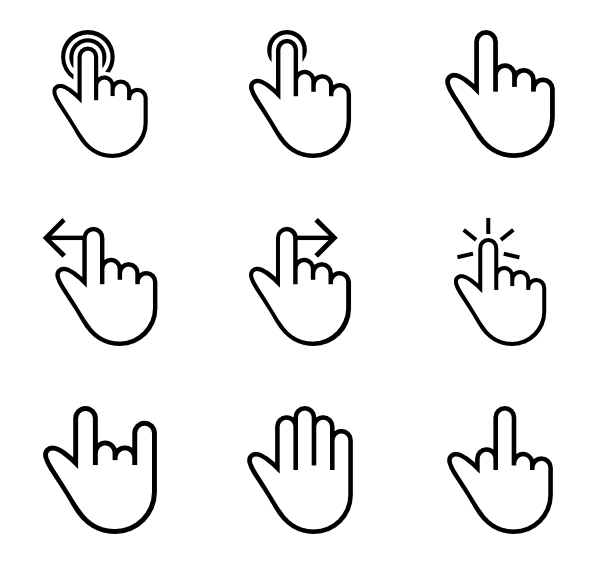
\includegraphics[width=10cm]{img/gesture}}

\begin{document}

%% Create title using header page information above
\maketitle

%% Table of Contents
\tableofcontents

%% List of Figures
%%\listoffigures

\pagebreak

\paragraph{Abstract}
Gesture-based UI has come a long way in the last 10 years. Gesture technology continues to grow slowly year over year with new technologies like Myo and Alexa taking the user interaction with the machine to the next logical solution. In this research paper, I will look into the history of user interaction with computers. Review gestures in everyday life and how gestures are used, and the modern age of gesture-based UI and the challenges faced by developers.

%% Section imports
\chapter{User Experience Evolution}

\section{Early Computers}
Computers and how we use them have changed dramatically as each generation is introduced to faster and better machines. How we interact with computers has changed drastically since the first electronic computers in the mid-1900s.

\begin{wrapfigure}{r}{0.5\textwidth}
  \begin{center}
    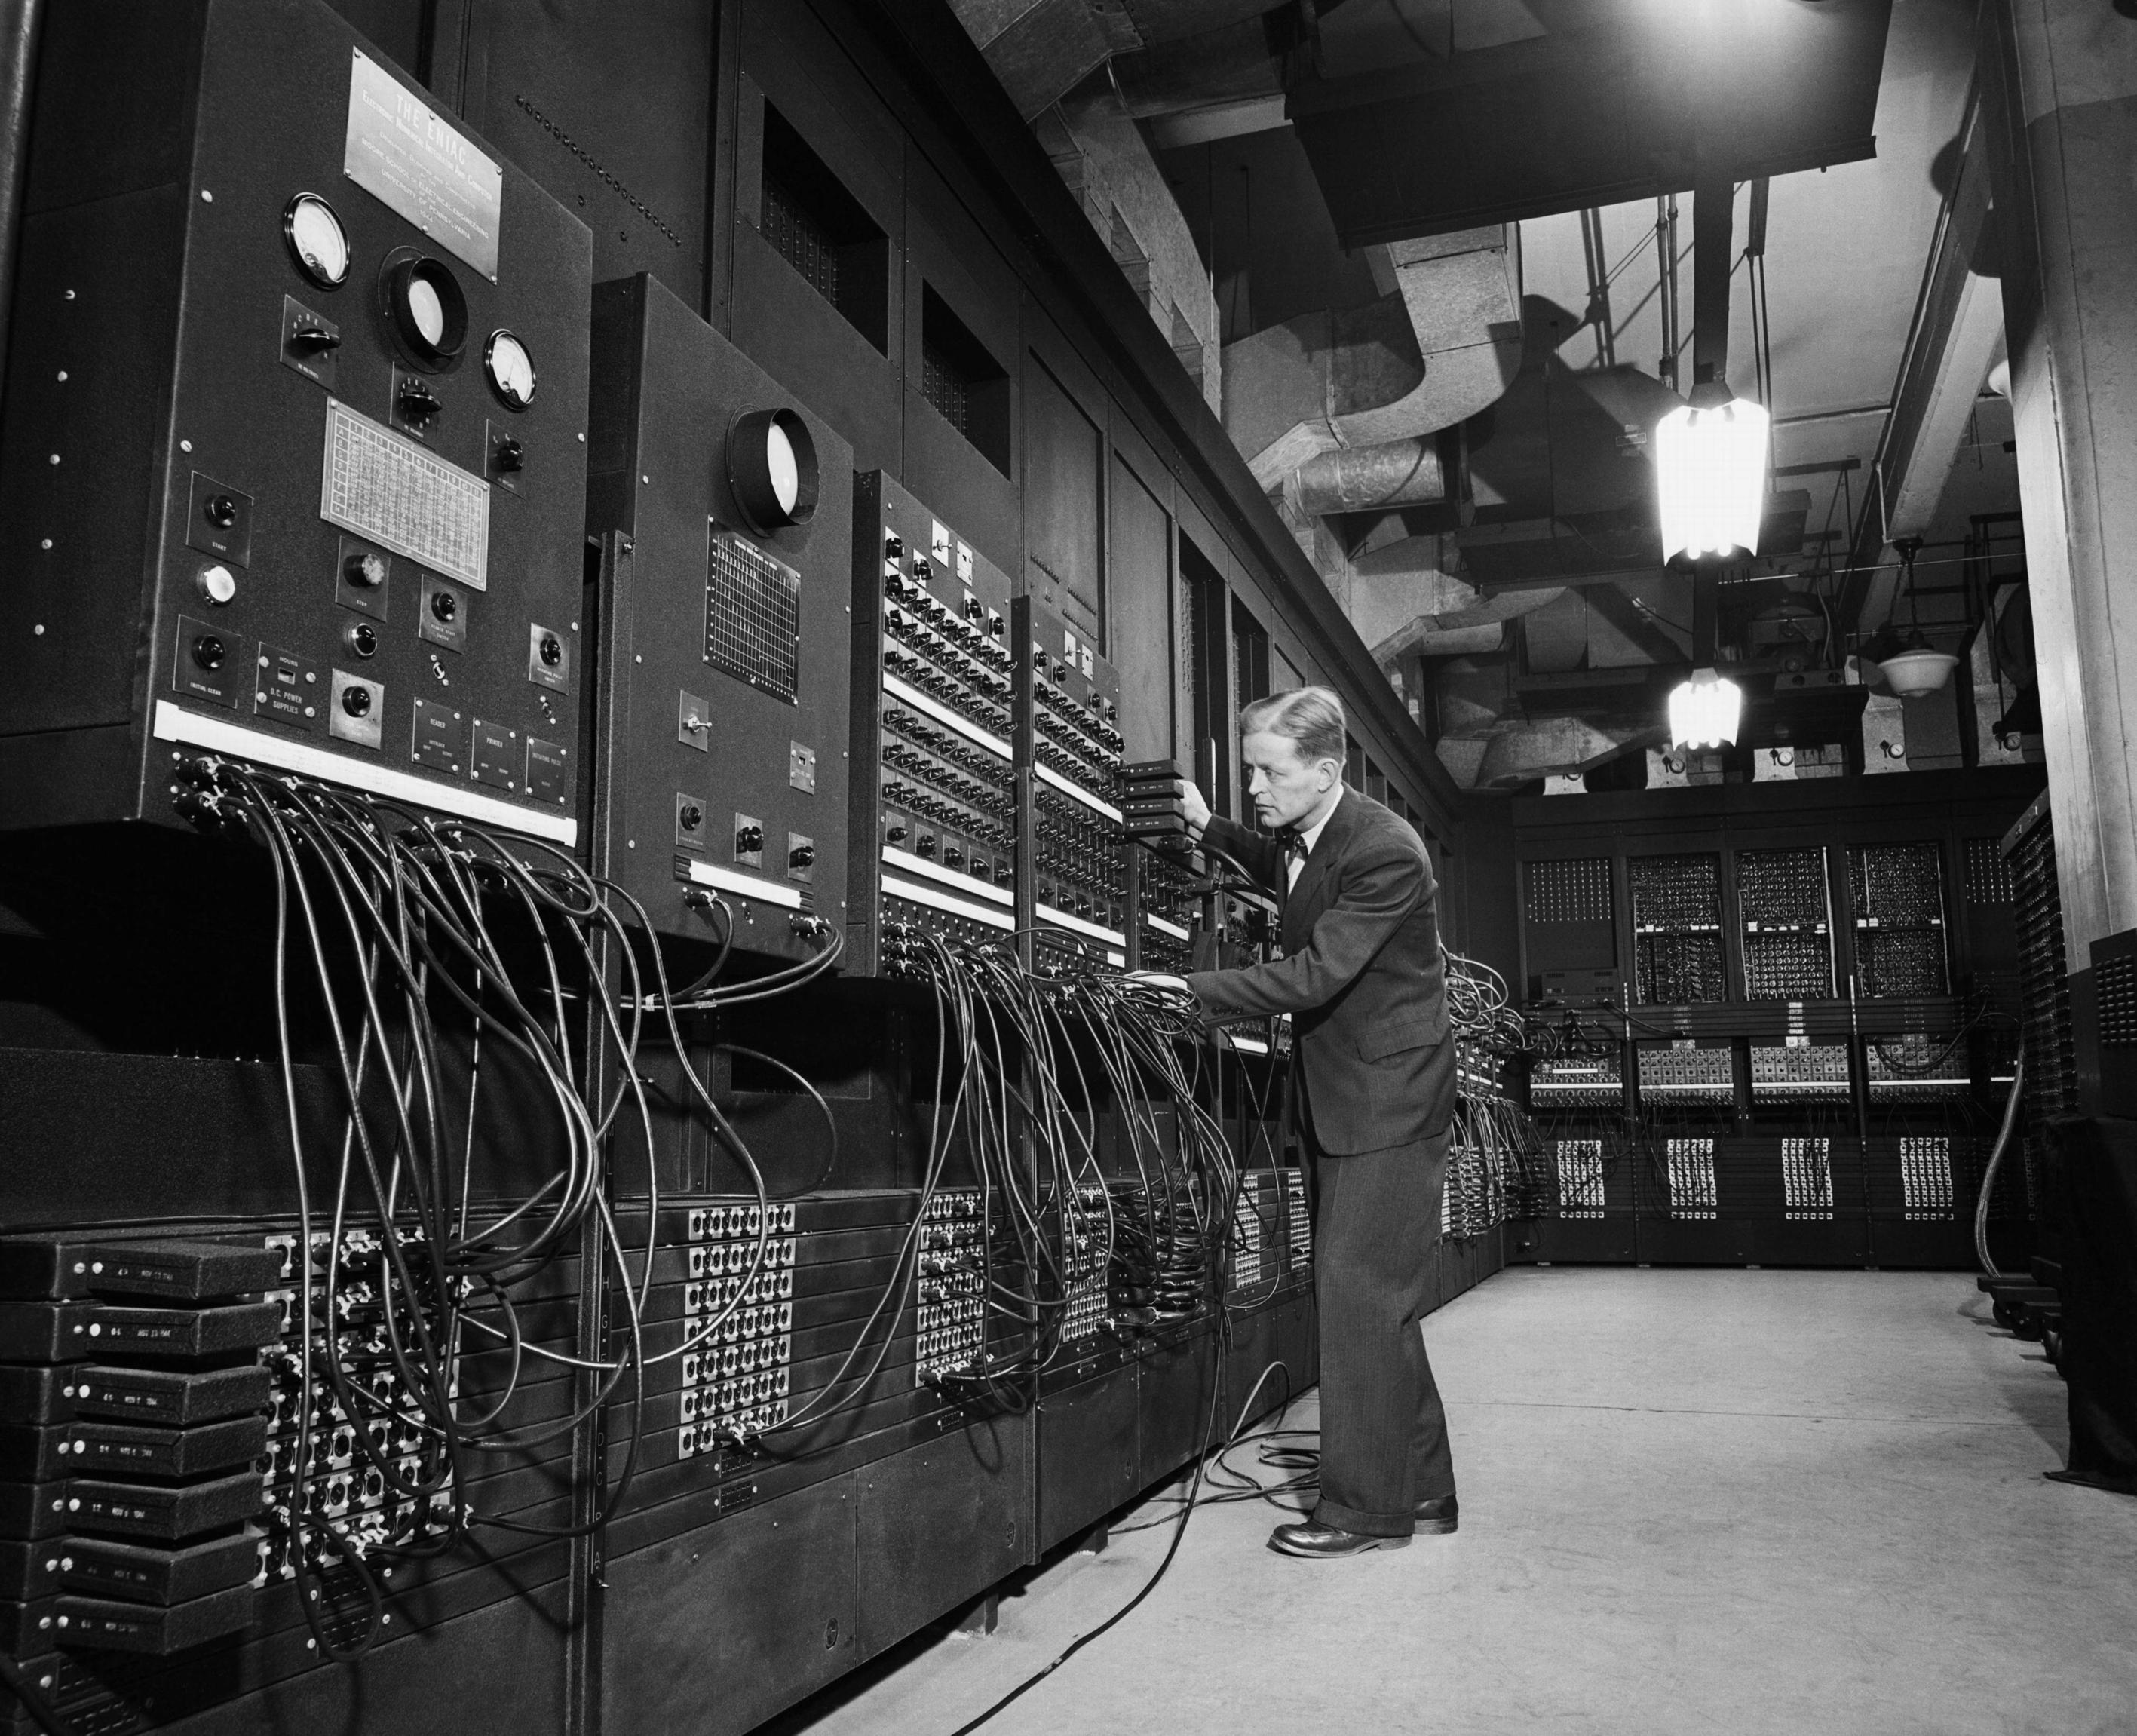
\includegraphics[width=0.48\textwidth]{img/eniac.jpg}
  \end{center}
  \caption{ENIAC}
\end{wrapfigure}

Early electronic computers such as the ENIAC (Electronic Numerical Integrator and Computer). \cite{eniac} The ENIAC was the first general purpose computer, this meant it could solve many problems as it could be programmed. The ENIAC was the first real step in user interaction with a computer, although the user had to have knowledge of the machine first, they could still operate it using over 3,000 switches and wires which could change how the machine made calculations. \cite{eniac} Although a primitive method of user interaction with a machine, it was the first 'modern' computer which the user had some control over its operation and change its operation by interaction.

Moving on from the ENIAC new computers were built with observations on how to improve over the ENIAC. Machines like the Manchester Baby \cite{manchesterbaby} allowed programs to be saved which was a huge leap in user intractable computers. Once a program was created by a programmer of the machine they could be saved and used again at a later date. This was a big step over the ENIAC where it took time to reprogram the machine each time they wanted to compute a specific task.

\section{}

\chapter{Gestures as a communication tool}
\chapter{Challenges for Design of Applications}

The biggest design challenge for developers of gesture controls is market adoption, standardization and gesture choice. From getting users to use the technology to make the technology comfortable to use on a daily basis. Developers both in hardware and software face many challenges in developing with this technology.

\section{Market Adoption}

\subsection{Myo Armband}

\begin{wrapfigure}{r}{0.5\textwidth}
  \begin{center}
    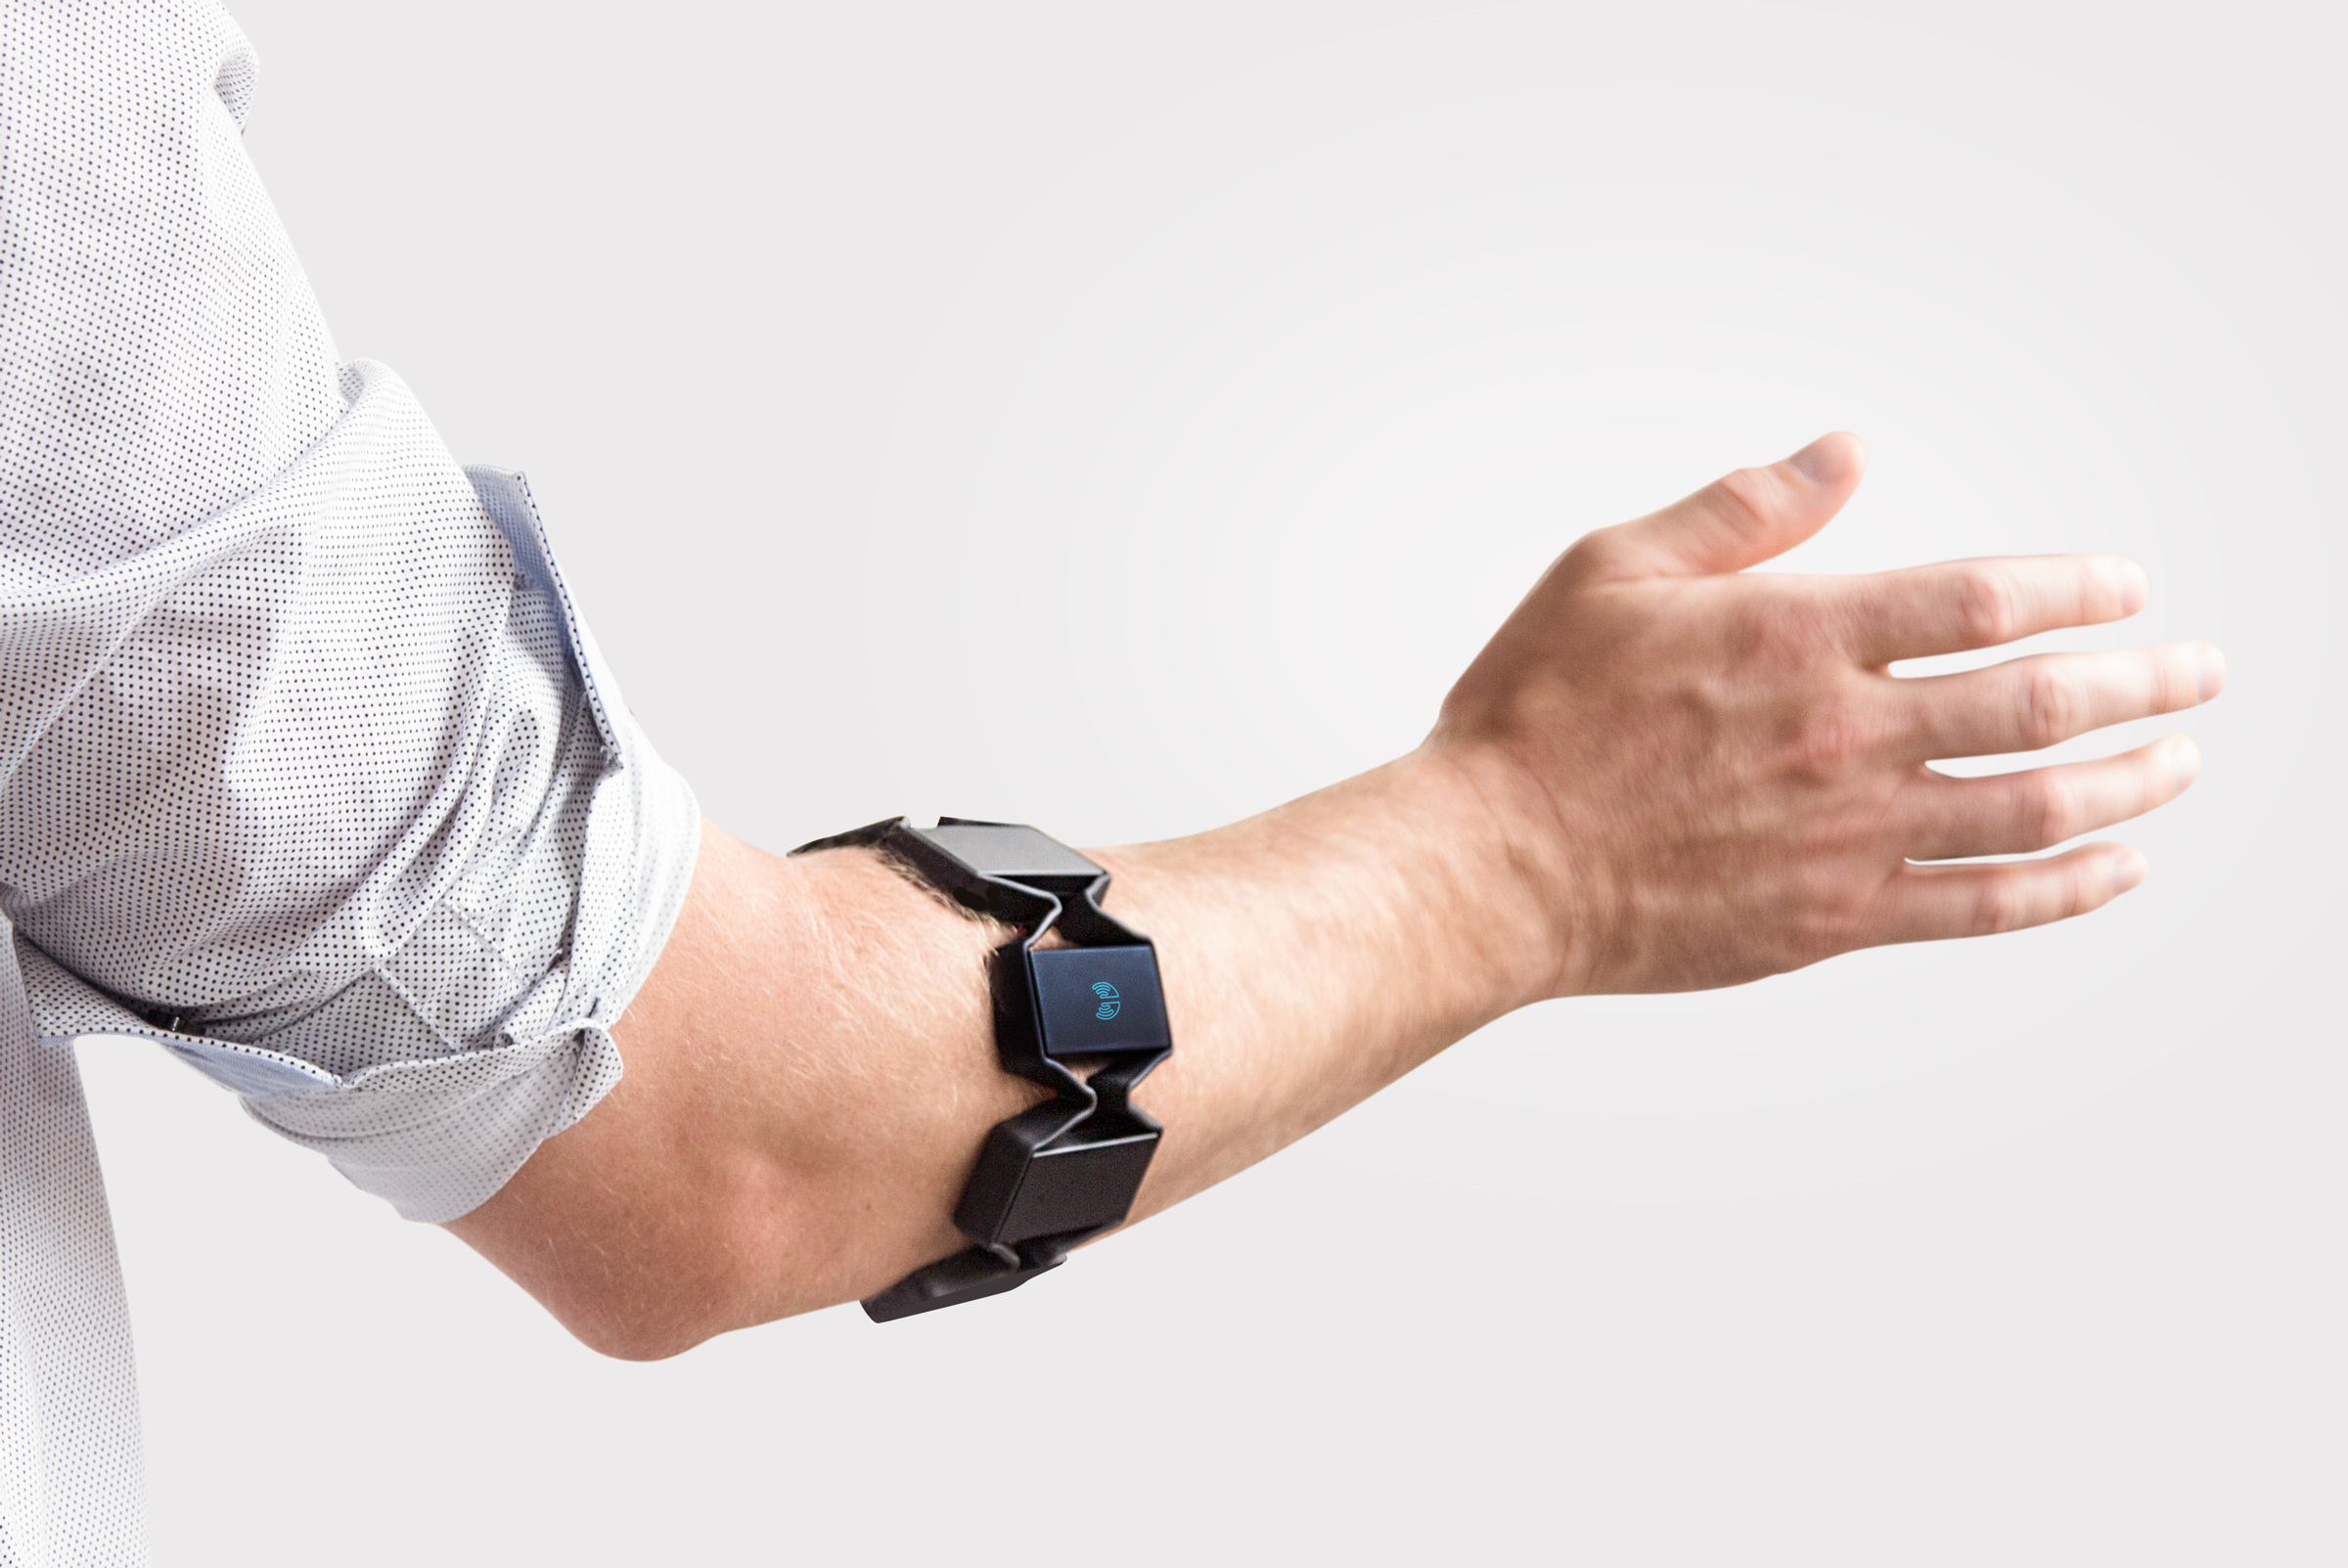
\includegraphics[width=0.48\textwidth]{img/myo.jpg}
  \end{center}
  \caption{Myo Armband}
\end{wrapfigure}

One of the biggest challenges of gesture-based technology is market adoption. If the technology isn't adopted by a large segment of the population developers mostly ignore it in favour of a bigger market, such as mobile phones and the traditional desktop.

Devices like the Myo armband started out with great success raising 14.5 Million dollars in 2013 with 30,000 pre-orders for their product. The problem started with lacklustre support from developers who weren't as supportive of the technology as the customers were. \cite{myosales}

Devices like Myo Armband suffered due to developer support which caused customers to lose interest with the technology.

\subsection{Kinect}

Even industry giant Microsoft tried to break into the gesture controls space with the introduction of the Kinect back in 2010. \cite{kinect} The Kinect was Microsoft's attempt of adding gesture controls to their gaming console the Xbox 360. With support from Microsoft, many developers made Kinect only games (Kinect Sports, Kinect Adventures!, Kinectimals) and other added Kinect support (Elder Scrolls: Skyrim, Forza Motorsports 4). With support from Microsoft, the Kinect looked to be on the rise as sales reached 10 Million. \cite{kinectsales}

\begin{figure}[H]
  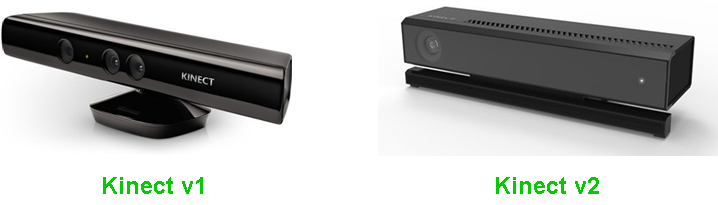
\includegraphics[width=\linewidth]{img/Kinect.png}
  \caption{Kinect V1/2}
  \label{fig:KINECT}
\end{figure}

From 2010 (Release of Kinect V1) to 2013 (Release of Kinect V2) customers opinion had changed on the Kinect. Many felt the Kinect games felt gimmicky' and games that added Kinect support didn't make using it over a traditional controller better. This dislike of gesture controls came to ahead with the release of the Xbox One, which originally was debuted with a new Kinect, which had to be plugged in at all times. With a price tag 100 dollars more than their competition, many blamed the Kinect for this price difference. 

With the Xbox One release having a Kinect market adaption should have been even better than the previous iteration of the Kinect. Unfortunately, the announcement of the Xbox One was a disaster causing lots of controversies that was then directed towards the Kinect. The Kinect got lacklustre support and many had a concern of privacy with an always-on camera and speaker. The Kinect was dropped in later models of Xbox Ones with users having to buy an adapter to get one to work with the newer models. This adapter was then dropped leaving users who enjoyed the connect behind.

\section{Standardization}
A huge problem with gesture controls is standardizing the technology involved. Each company makes its own proprietary technology which leads to lacklustre developer support if the consumer-base isn't high enough. An example is the Xbox Kinect. The Kinect got support from Microsoft with games only for Kinect, which is fine as the game is developed by Microsoft. The problem with support comes from third party companies. These companies want the biggest profit they can get and by creating a Kinect only game it restricts their consumer-base to Kinect only users. Companies would rather release on both Xbox and PlayStation and add in Kinect features. The problem with this style of development is it leads to these Kinect features being thought of after the game has already been made, leading them to be pushed to the side as 'gimmicky' by consumers.

Microsoft is trying to create a standard using their Microsoft Launcher on Android Phones. By allowing the user to customize what gestures do for them, making the gestures more comfortable for the user and by putting this feature on the Android Play-Store giving users around the world access to this feature set.

\section{Gesture Choice}
During the development of gesture-based technology, the developers need to be wary of how the gestures are used. Gestures that mean one thing here means something else over there, so if developers aren't careful they can be met with lots of criticism. A huge part of gesture development is researching the gesture controls to see which gesture would fit best for a particular action.

With less and fewer buttons on phones, many developers have to keep gestures in mind when developing applications for phones. Luckily both Android and iPhone share similar designs allowing developers to carry these gestures across devices, hitting a larger market of users. Phones are a word wide item used by billions. Many people take gestures on phones for granted as we become accustomed to them. If an application doesn't support basic gestures such as swiping up and down to navigate it can make it feel quite old and awkward to use so many will just not use it.

An important part of developing gestures for users is to keep some sort of standard. Many expect to be able to swipe up and down to navigate with one finger, changing this to require two for your application will annoy user away from it. This is why hardware manufacturers like Apple will include how developers should handle certain gestures. 
\chapter{Challenges for Implementation}
Tracking users with gesture-based technology is one thing, interpreting whether the intended function is meant in another thing. Intent and context is integral to human interaction and especially when using gestures. Intent and context is a very important part of gesture technology moving forward.

\section{Voice Controls}
\subsection{Context and Intent}

\begin{wrapfigure}{r}{0.5\textwidth}
  \begin{center}
    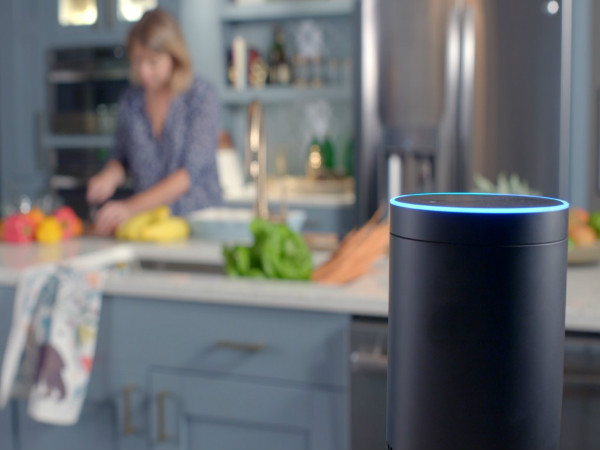
\includegraphics[width=0.48\textwidth]{img/alexa.jpg}
  \end{center}
  \caption{Alexa Active}
\end{wrapfigure}

A big problem with voice controls is interpreting whether the user is trying to enact a function or the user is just talking to another person. Alexa, for example, will commonly mistake the two people talking about Alexa for them trying to interact with the device. The Alexa machine has difficulty understanding the context of the conversation and activates when hearing the keyword being spoken. This keyword is used to activate the device with the remaining speech being the function the user wishes to enact. Manufacturers are still trying to grasp when the user is talking about the device or trying to use it. Basic workaround such as Calling the device Google Assistant and making the wake word 'Hey Google' is a basic workaround which has worked for Google, but failed for Amazon. Amazon customers often complain their home assistant thinks they're trying to use it when they are just talking about it. This is a problem with how Amazon advertised their devices under Amazon Alexa and Alexa Compatible which has caused the user to think of the entire device as Alexa rather than an Amazon Echo with Alexa built in.

\subsection{Interpreting Intent}
Interpreting what the user wants is a hard task. There are many ways of phrasing sentences and figuring out what the user is trying to do is a challenging task.

Devices like Amazon Echo have three major methods of figuring out user intent. Alexa will separate a phrase into three parts.

\begin{itemize}
    \item Intents
    \item Slots
    \item Slot Types
\end{itemize}

The three parts help break down a sentence and figure out what the user wants the device to do. 'Intents' are like functions in programming, 'Slots' are the variables and 'Slot Types' are the variable types. Using these three parts Alexa can break the sentence down and figure out what has to be done. For example, if the user says 'What is one plus two',
Alexa will use the sentence to find an Intent that best matches what the user has asked. Once found Alexa will get the slots in the sentence. The slots are 'one' and 'two'. Alexa will then use slot types to figure out what the slots are. Slot types are numerous ranging from numbers to German cities to American politicians. With the slot type, Alexa can figure out what is being said. Using the slot type in this example Alexa will figure out that 'one' and 'two' are numbers and return '1' and '2' instead of the string representation. Using this method Alexa can figure out most of the user requests.

\section{Physical Controls}

Tracking physical gestures is very tricky because unlike voice gestures there is no wake word to recognize tracking and cease after the function has been enacted. 

\begin{wrapfigure}{r}{0.5\textwidth}
  \begin{center}
    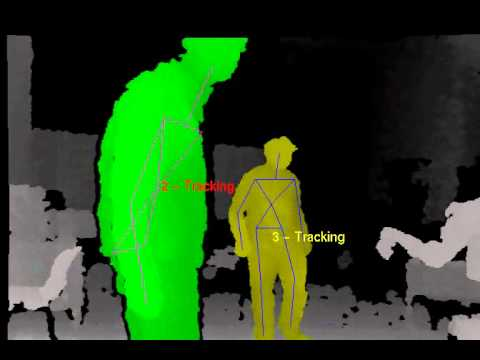
\includegraphics[width=0.48\textwidth]{img/kinecttracking.jpg}
  \end{center}
  \caption{Kinect Tracking}
\end{wrapfigure}

Microsoft's Kinect for example, its tracking works be imposing a digital skeleton onto the users in the frame in order to track location and limb movement. This method makes for accurate tracking of the entire body and can slowly be expanded upon while also being compatible with previous games and applications. 

Microsoft's Kinect is an extremely accurate gesture tracking technology which has been adapted to work in industries beyond its core gaming focus. But its accuracy may cause problems when the user wishes it to stop tracking. Microsoft has come up with multiple ways to fix the problem of gesture tracking when the user wishes to pause the software. The user can do a specific gesture to bring up the Xbox menu in order to pause the game and can use this gesture in order to return to the game. But the main method of interacting with menus and pausing or exiting an application is by using the built-in voice gestures on the Kinect. By using these voice gestures the user can still remain away from any physical input and control any application through gestures. The Kinect can turn on the Xbox console through voice gestures and then can be controlled through gestures both voice and moving your arm.
\chapter{Conclusions}
We are moving further and further away from traditional methods of interacting with computers. We've gone from having to use dials and wires, to using a keyboard and mouse. Between these two stages, there was a slow progression to make interacting with computers easier and require less and less knowledge of how a computer works. Gesture-based technology is the next step in human-machine interaction, the questions aren't if it'll happen, but when. In its current state gesture-based technology has faced issues with developer adoption, which ultimately leads to consumer dissatisfaction with the product. 

Gestures as a communication tool is one of the oldest methods of communication and will remain as long as two people can communicate with one another. The limitations in gesture technology in the intent and context behind the gesture. Human language requires context and is full of innuendos, which carries over to gesture-based communication. These small innuendos are hard to teach machines, so in the current generation, workaround needs to be used in order to fix this small problem.

Ultimately gesture controls will replace interaction with a computer for most people. The challenge comes with adoption rate with physical gestures as voice gestures are being implemented into device users are already familiar with and have such as smartphones.

\printbibliography
\end{document}